\section{Historique des calculateurs}\label{sec:von}


Bien que leur architecture des processeurs ait beaucoup évolué depuis leur création, l’organisation globale n’a pas changé. Aujourd’hui la majorité d’entre eux sont basés sur une architecture qui porte le nom  du scientifique à l’origine des premiers schémas : l’architecture \textit{Von Neumann}.

\subsection{Les premiers calculateurs}

L'origine des premiers calculateurs remonte bien avant l'invention des systèmes électroniques. Les premières machines à calculer sont apparues à la fin du 16e siècle, conçues par Blaise Pascal et Gottfried Wilhelm Leibnitz \cite{Vie1996}. Les opérations en base 10 étaient à réaliser par l’utilisateur au moyen de roues dentées. 
Pour automatiser le recensement des 62 millions d’Américains vivant aux États Unis en 1890, le gouvernement lança un appel d’offres pour construire un système de traitement automatique. Herman Hollerith proposa alors d’utiliser un système de cartes perforées utilisé par des sociétés ferroviaires produit par la société Computing-Tabulating-Recording.  C’est en 1924 que la société fut renommée  International Business Machines (IBM). DE 1937 à 1943, IBM construit pour l’Université de Harvard un calculateur géant capable de multiplier deux nombres de 23 chiffres en six secondes appelé  Automatic Sequence Controlled Calculator (ASCC) \cite{cortada2016computer}. Cet ordinateur fonctionnait à partir de dispositifs mécaniques et électromécaniques issus des machines à cartes perforées.

Un autre projet de recherche à l'origine de l'ordinateur est celui mené par Allan Turing durant la Seconde Guerre mondiale. Utilisés pour décoder les messages chiffrés d'Enigma utilisée par l'armée allemande. Le câblage de ces premiers automates devait être refait lorsqu'on voulait appliquer un changement dans le traitement des opérations. On parlait alors de programmes extérieurs. Le calculateur d'Allan Turing avait une seule utilité, non des moindres, celle de déchiffrer des messages. Il ne pouvait cependant pas être utilisé pour réaliser d'autres calculs.

En 1945, Von Neumann proposa les 3 premiers principes qui sont à l'origine des ordinateurs actuels. Le premier voulait que ces machines soient universelles, c’est-à-dire qu’elles puissent exécuter différents types de calculs. Le deuxième concernait leur programmation: on parle alors d’instructions organisées dans des programmes qui, comme les résultats intermédiaires, peuvent être sauvés en mémoire. On parle alors de programmes enregistrés. Le troisième principe est l’implémentation de la rupture de séquence. Lors de l’exécution d’un programme, l’automate décide des instructions à exécuter, réalise des tests et des comparaisons pour faire des sauts dans le programme. 


\subsection{L'architecture Von Neumann}

C'est en 1945 que cette architecture a été présentée pour la première fois par John von Neumann dans un papier qu'il n'aura pas le temps de finir \textit{First Draft of a Report on the EDVAC}. Cependant, sur ce papier ne sont pas mentionnés les deux autres contributeurs que sont J. Presper Eckert et John Mauchly. Malheureusement pour eux, l'histoire ne retiendra que le nom du premier. Leur papier décrit une façon d'organiser un système électronique dans le but d'exécuter des instructions. La principale idée de cette architecture est la présence de trois modules principaux (voir \autoref{pic_cpu_von}):
 \begin{itemize}
    \item Une unité de traitement (CPU) qui contient une unité arithmétique et logique (ALU) qui s'occupe d'exécuter les opérations de bases (addition, multiplication, etc.) ainsi que de registres pour mémoriser les données utilisés pour leur exécution.
    \item L'unité de contrôle qui lit les instructions et organise leur exécution en s'occupant de demander les données nécessaires à la mémoire.
    \item Une mémoire qui contient toutes les données, mais aussi le code à exécuter contrairement aux anciennes architectures qui lisaient les programmes sur des cartes perforées, rubans, ou tableaux de connexion.
 \end{itemize}


\begin{figure}
    \centering
    \begin{subfigure}[b]{0.45\linewidth}
        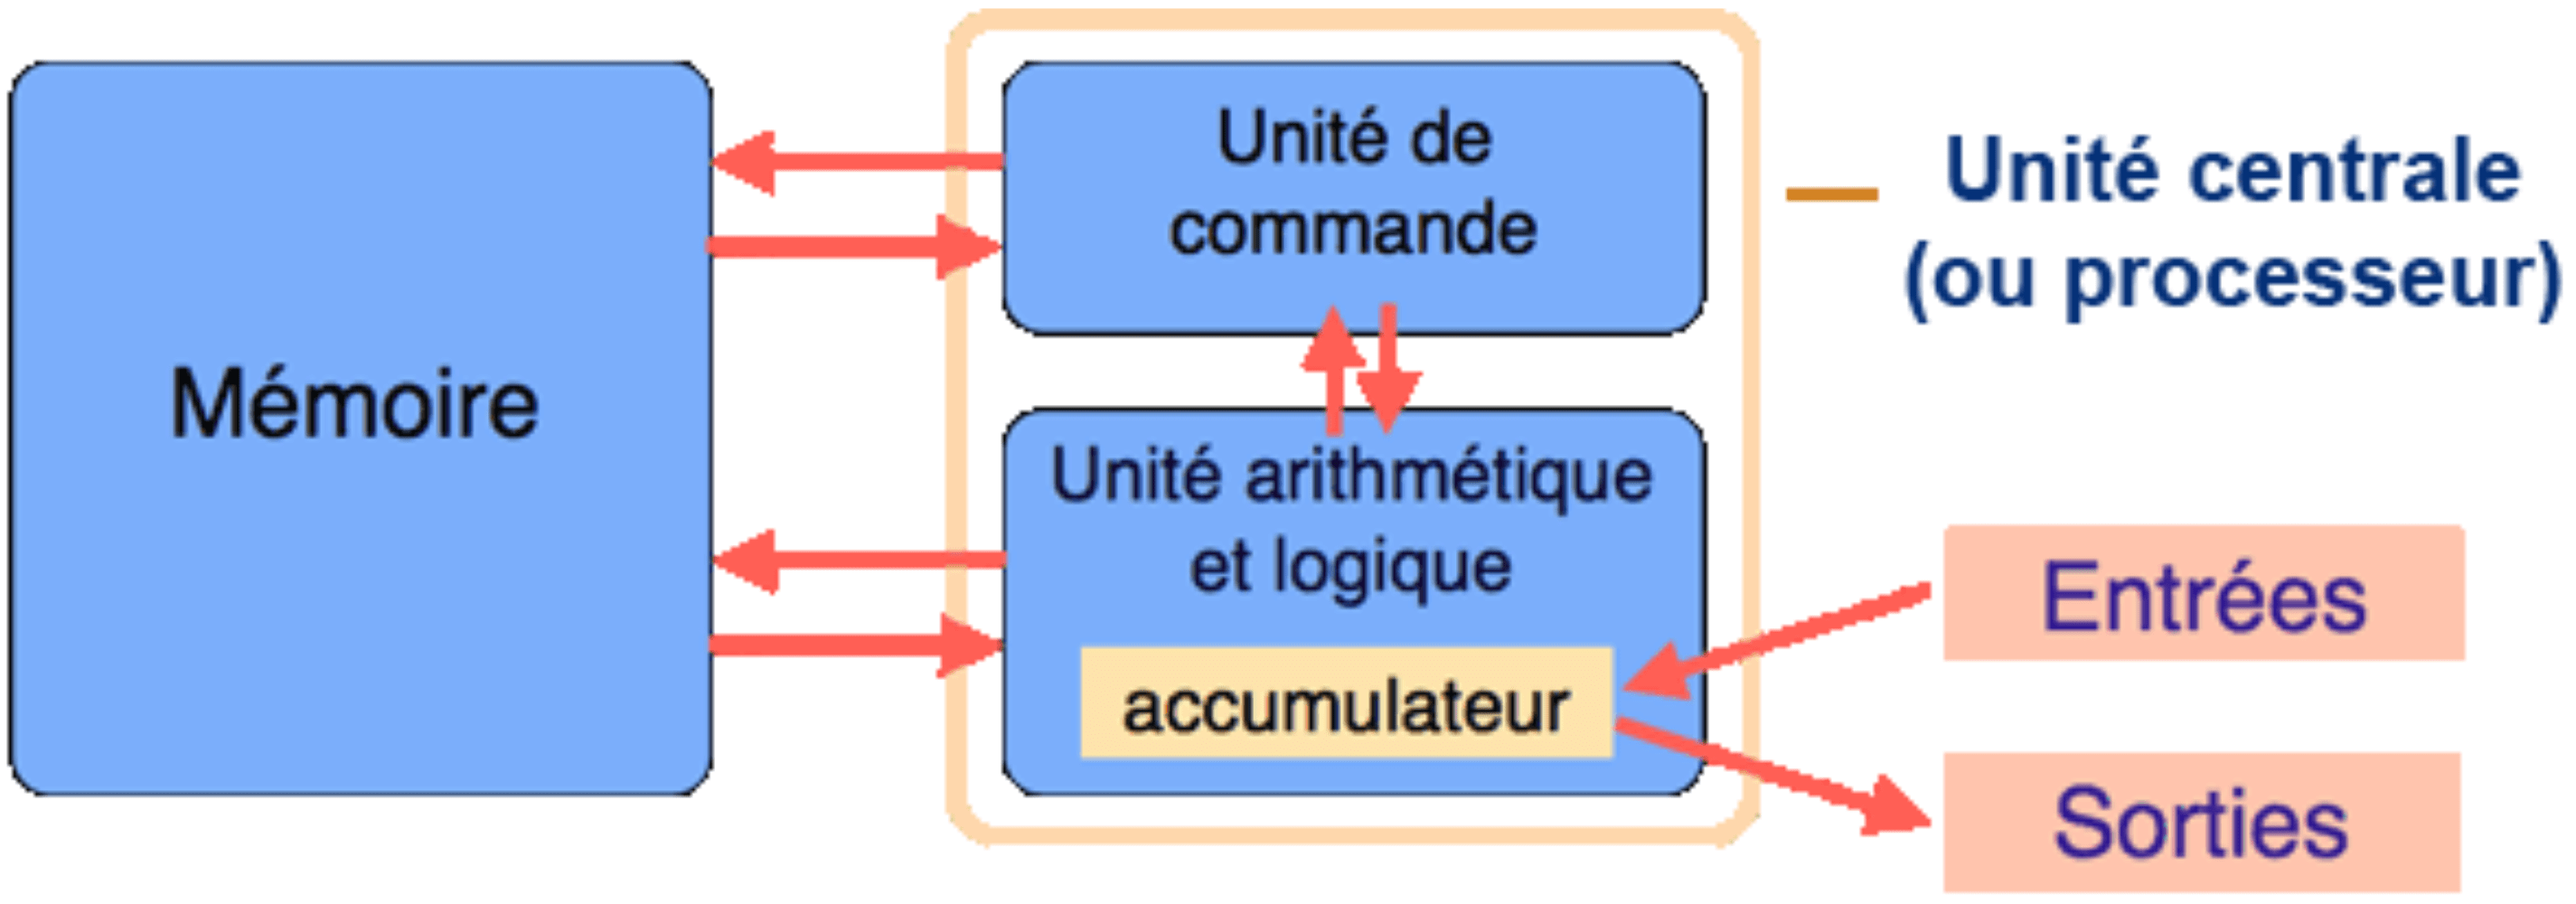
\includegraphics[width=\linewidth]{images/cpu_von1.png}
        \caption{Architecture Von Neuman initiale}
        \label{pic_cpu_von}
    \end{subfigure}
    ~ %add desired spacing between images, e. g. ~, \quad, \qquad, \hfill etc. 
      %(or a blank line to force the subfigure onto a new line)
    \begin{subfigure}[b]{0.45\linewidth}
        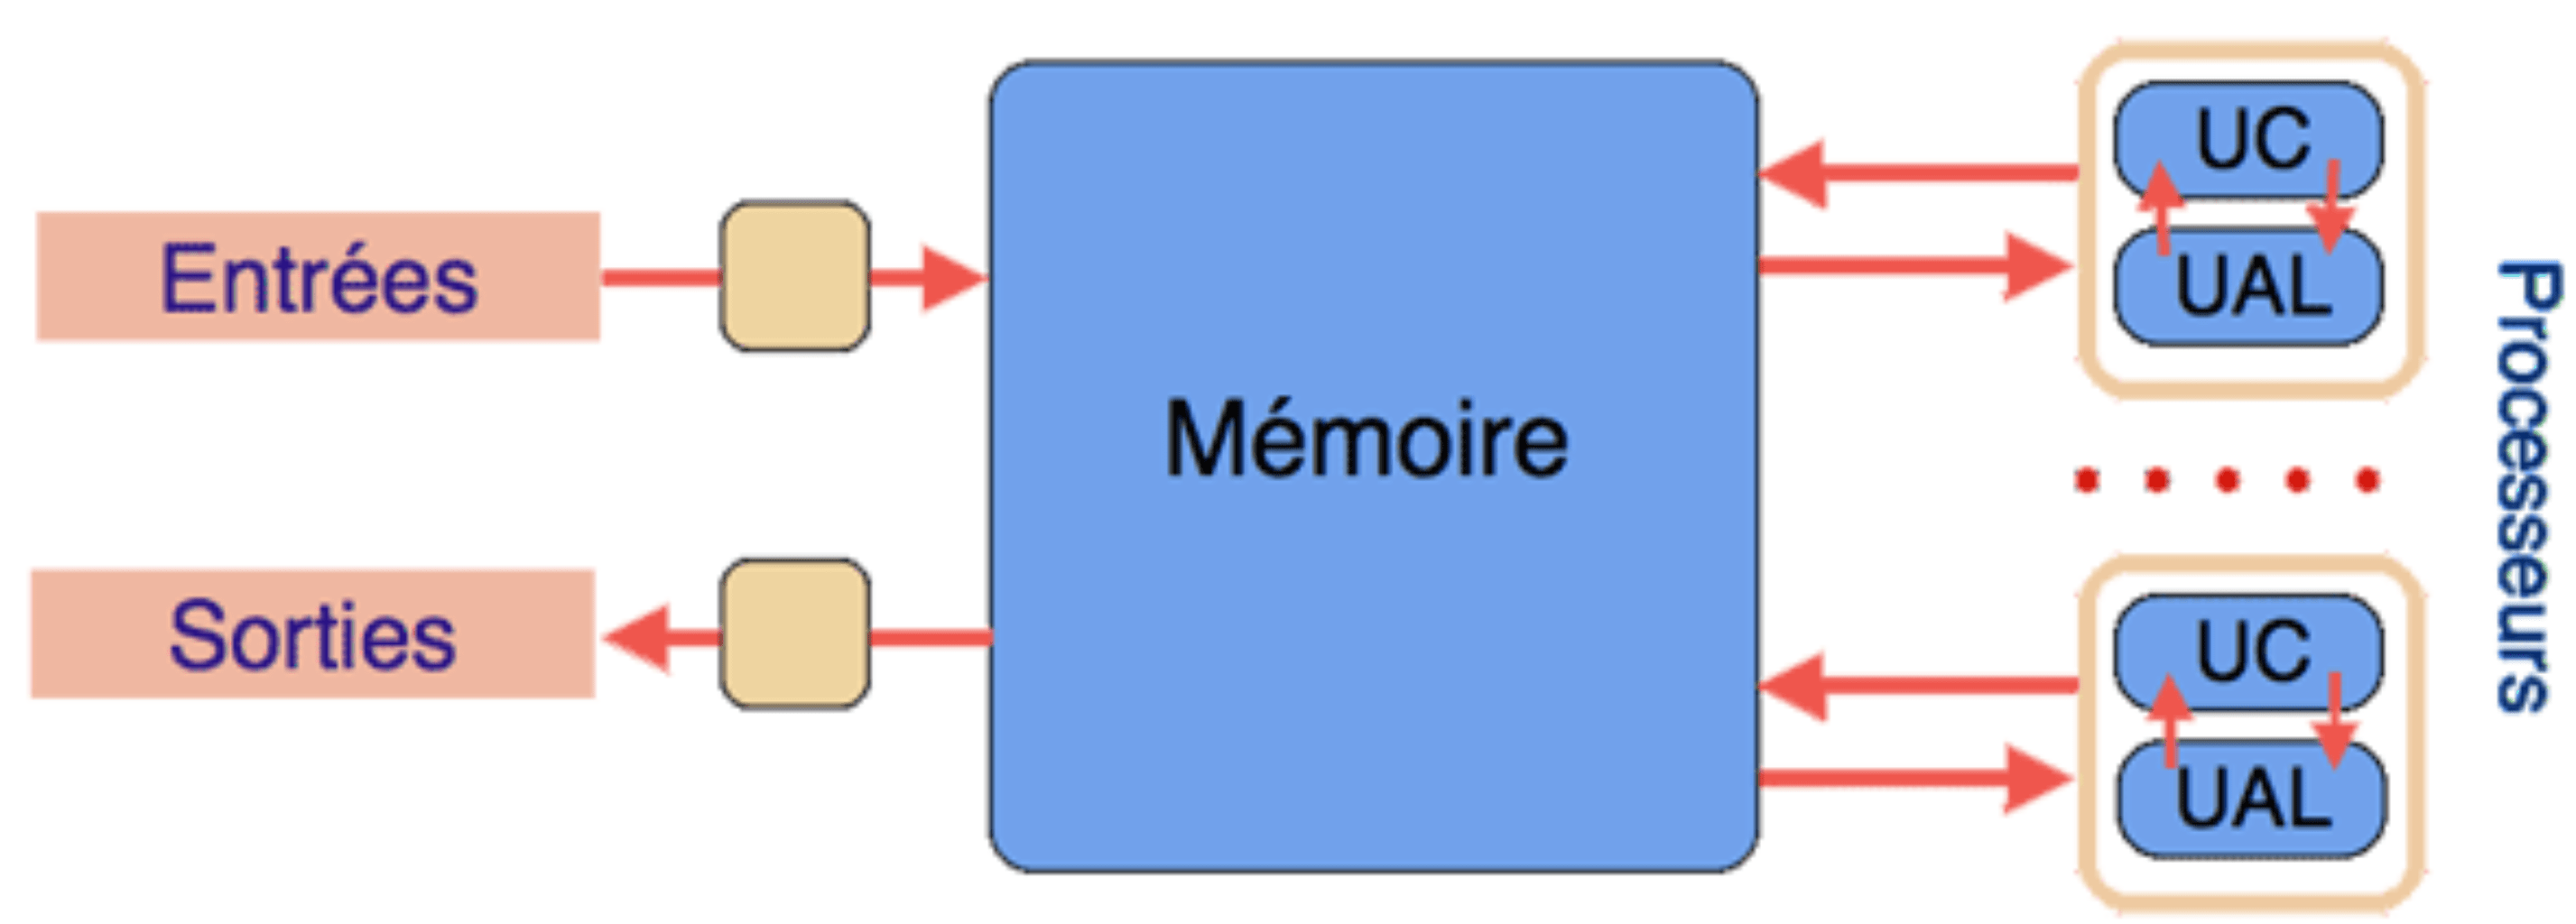
\includegraphics[width=\linewidth]{images/cpu_von_new.png}
        \caption{Quelques évolutions de l'architecture}
        \label{pic_cpu_von2}
    \end{subfigure}
    \caption{Architecture Von Neumann\protect\footnotemark }\label{fig:cpu_archi_von}
\end{figure}

\footnotetext{source: https://interstices.info/le-modele-darchitecture-de-von-neumann}

Bien que l’implémentation de cette architecture ait évolué avec l’apparition de nouveaux matériaux, les architectures modernes des processeurs sont toujours construites sur ce modèle. Deux évolutions de l’architecture initiale ont cependant été appliquées (\autoref{pic_cpu_von2}). Les entrées et sorties ne sont plus gérées directement par l’unité centrale, mais par des microprocesseurs dédiés. L’unité centrale de traitement n’est plus unique depuis l’apparition des processeurs multicoeurs. Ces évolutions ne remettent pas en cause les principes de bases énoncés par Von Neumann. 


\subsection{Architecture Harvard}\label{sec:harvard}

Dans leur papier \cite{238389}, Von Neuman et al. précisent que la façon dont sont stockées les instructions et les données en mémoires doit être la même. Cette configuration la différencie de sa principale concurrente, l'architecture  Harvard (figure \ref{pic_neumannHarvard}) qui utilise deux bus pour accéder à deux mémoires réservées l'une pour les instructions, l'autre pour les données. 
Cette configuration permet à l'architecture Harvard d'accéder en parallèle aux données et aux instructions. De plus, comme les instructions et les données sont séparées, elles peuvent être stockées sur des supports de différentes performances. On peut ainsi utiliser un support plus cher pour stocker les données avec des mémoires très rapides (SRAM) et stocker les instructions sur des mémoires moins chers de type ROM. De plus, l’architecture Harvard apporte une sécurité en empêchant les processeurs d’exécuter des instructions provenant du stockage réservé aux données. Enfin la nécessité d’avoir deux bus rend les puces Harvard plus chères et les performances sont souvent moins bonnes. Un code qui aurait beaucoup d’accès mémoire ne pourrait pas profiter de la disponibilité du canal allant à la mémoire des instructions. Dans une architecture Von Neumann à deux canaux, les bus peuvent être utilisés aussi bien pour des instructions que pour les données. Cependant la performance de ce bus mémoire est à l’origine du déséquilibre de performance des architectures modernes. Ainsi, il est courant d’utiliser le terme de \textit{goulot de Von Neumann} pour désigner ce point faible des architectures modernes.

\begin{figure}
    \center
    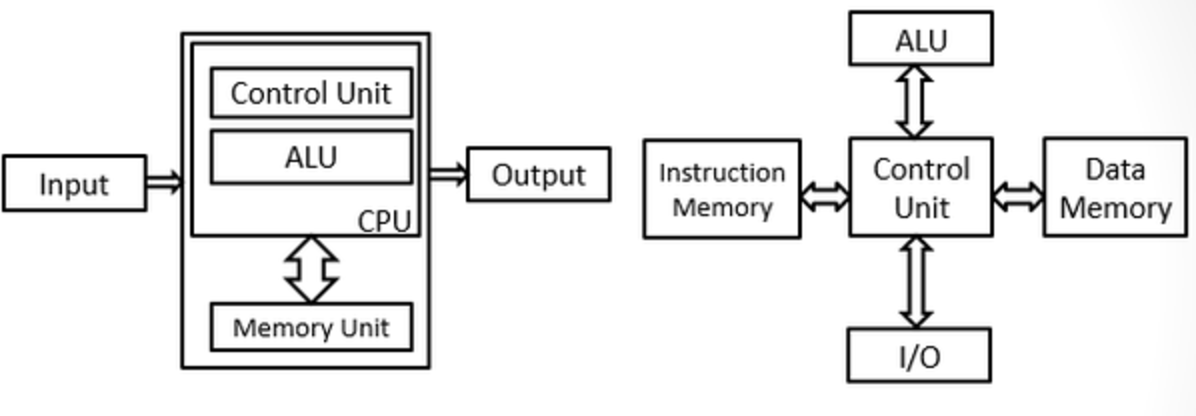
\includegraphics[width=10cm]{images/Chapitre1/neumannHarvard.png}
    \caption{\label{pic_neumannHarvard} Les deux principales architectures de processeurs: Von Neumann et Harvard. }
\end{figure}